\chapter{Materials and Methods}

%This section is to clarify the pre-existing tools, defining what was developed in this field until now, and why this tool was used instead of others.

%The general structure is the following:
%\begin{itemize}
%	\item Definition of the specific tool(s) studied (robots, sensor nodes, smart-phones). When relevant, pre-existing experiments.
%	\item Definition of the context of use (indoor/outdoor, humans/animals/robots, with/without connection).
%	\item Definition of used protocols (How the data are collected, when, etc.)
%\end{itemize}


This Chapter introduced the background and state of the art on multi-robot task scheduling. Chapter \ref{sec:ros_concepts} introduces important concepts of ROS. Chapter \ref{sec:modeling_gazebo} introduces the 3D modeling of robot and environment in Gazebo. Chapter \ref{sec:navigation} introduces robot navigation. Chapter \ref{sec:centralized_method} introduces exist task scheduling methods. Chapter \ref{sec:distributed_method} introduces distributed methods. Chapter \ref{sec:cost_function} introduces the cost funtion methods.

\section{Important Concepts of ROS}
\label{sec:ros_concepts}
The ROS Wiki \cite{ros} defines ROS as an open-source, meta-operating system for your robot. It provides the services you would expect from an operating system, including hardware abstraction, low-level device control, implementation of commonly-used functionality, message-passing between processes, and package management. It also provides tools and libraries for obtaining, building, writing, and running code across multiple computers.
In another word, it is a robot software platform that provides various development environments specialized for developing robot application programs\cite{Pyo17}.

\subsection{Node}
A ROS node is the smallest unit of processor running in ROS. In another word, it is one executeble program. In this project, some existing special nodes are used. For example ``move\_base'' node provides a ROS interface for configuring, running, and interacting with the navigation stack on a robot. There are some nodes created for this project, and each node are created for different purpose, for example, one ``Robor controller'' node controls one robot. 

\subsection{Communication Infrastructure}
ROS has a built-in and well-tested messaging system. There are different methods to exchange messages.  ROS topic is a unidirectional anonymous communication. It is used when exanging data continuesly. The subscriber receives messages of publisher node only when both of them registered the same topic name. ROS service is bidirectional synchronous communication. The service client request a service and the service server responds to the request. The ROS action is a bidirectional asynchronous communication. It is used when it is difficult to use the service due to long response times after the request or when an intermediate feedback value is needed.
The diagram of message communication is shown in Figure \ref{fig:ros_message_communication}.  There are some utilization of message communication in this project. Chapter \ref{sec:sensor_simulatior} introduces the sensor simulation senario that utilizes ROS Topic method. Chapter \ref{sec:communication_protocols} introduces the communication protocols in this project that utilize ROS service method and ROS Action method.   

\begin{figure}
    \centering
    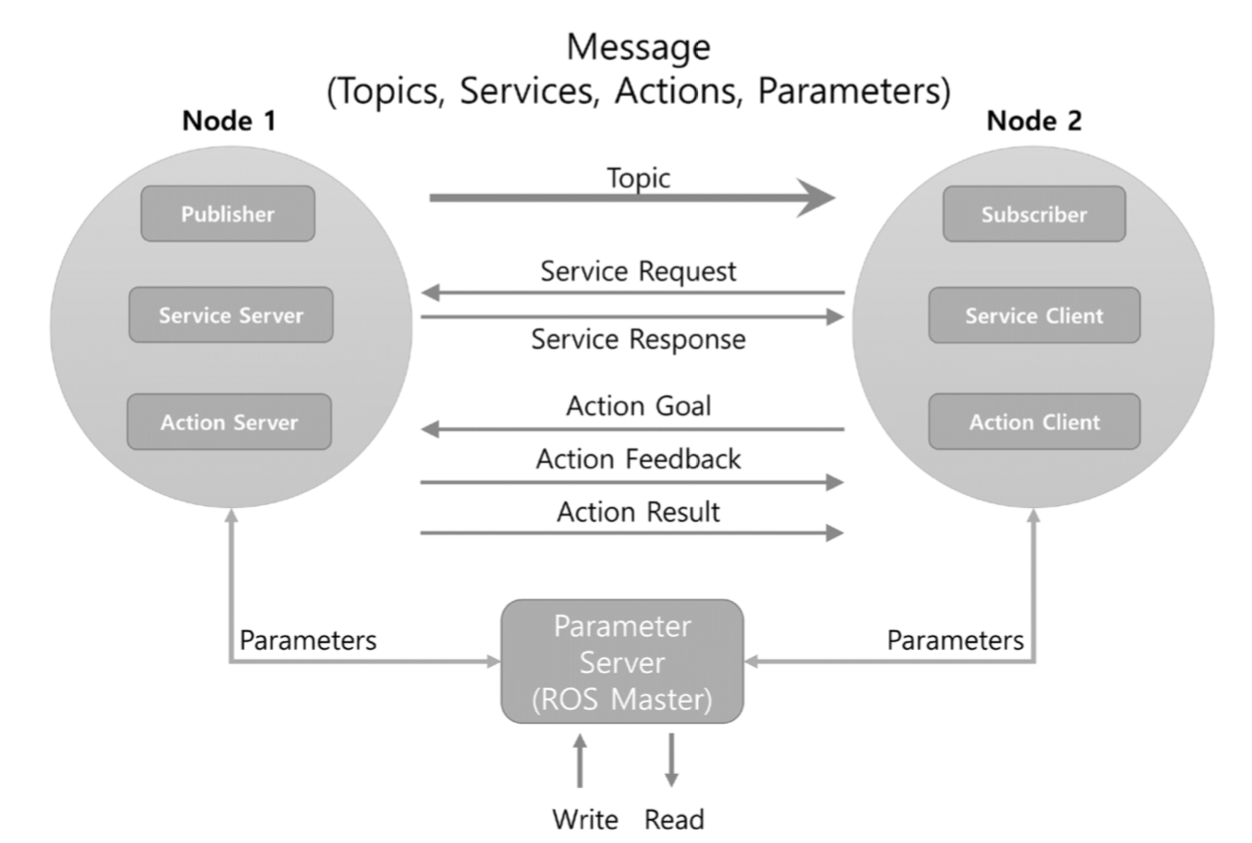
\includegraphics[width = 0.7\textwidth]{content/images/ch2/ros_message_communication.png}
    \caption{ROS Message Communication}
    \label{fig:ros_message_communication}
    \end{figure}
    
\subsection{ROS Tools}
ROS's core functionality is enhanced by a variety of tools and packages:

\begin{itemize}
    \item \textbf{Rviz.} Rviz\cite{RVIZ} is the 3D visualization tool of ROS. It can visualize information like the distance from a Laser Distance Sensor (LDS) to an obstable, image value obtained from a camera, Point Cloud Data (PCD) of the 3D distance sensor such as RealSense, Kinect, or Xtion. As is shown in Figure \ref{fig:rviz_gui}, multiple robot model and its path and laser data can be displayed.
    \begin{figure}[htbp]
        \centering
        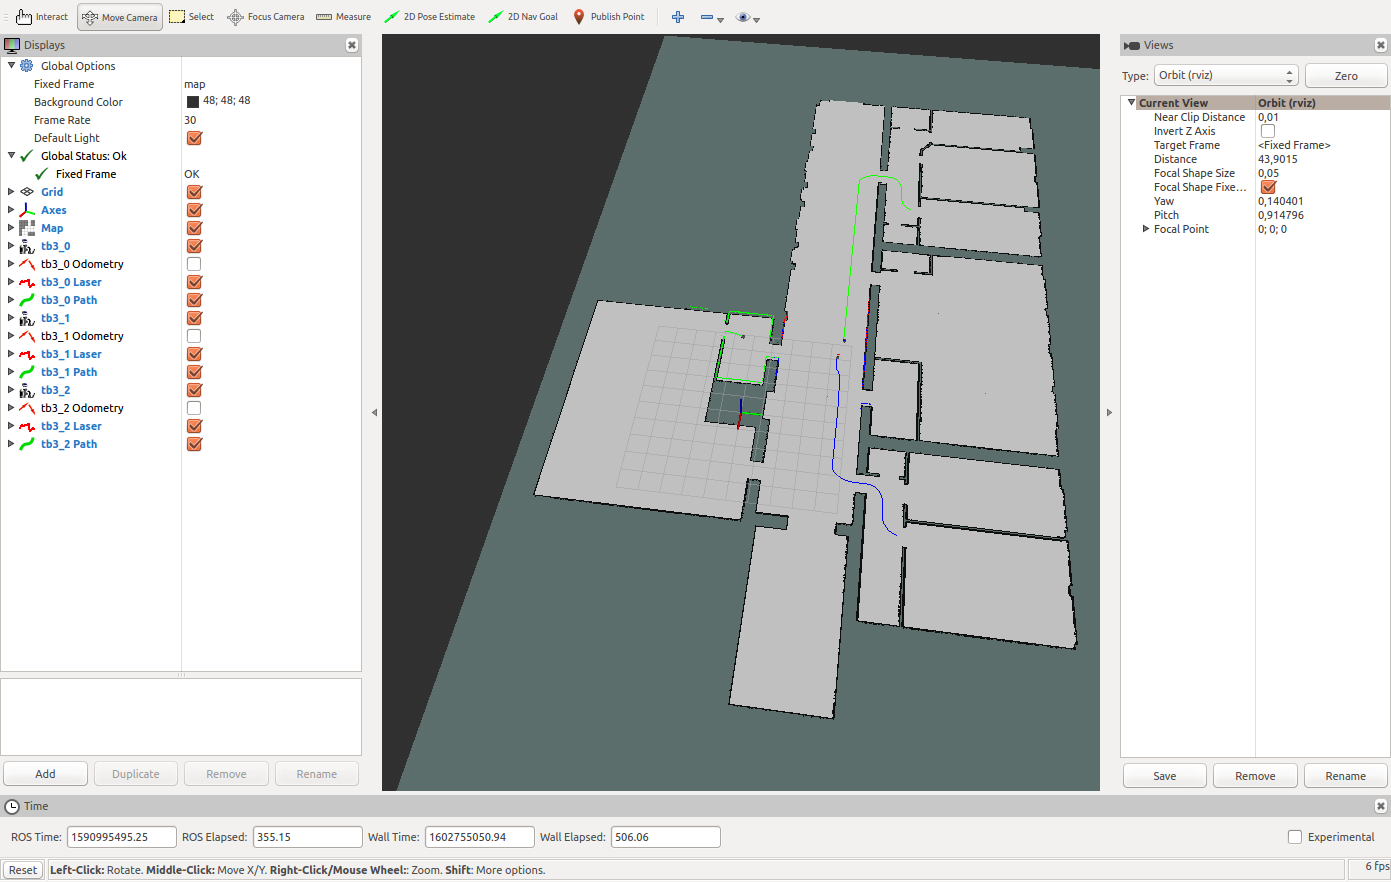
\includegraphics[width = 0.7\textwidth]{content/images/ch2/rviz_gui.png}
        \caption{Rviz Example: Navigaion using TurtleBot 3 and Laser Distance Sensor (LDS)}
        \label{fig:rviz_gui}
    \end{figure}

    \item \textbf{rqt.} rqt is an intergration of more than 30 Qt-based ROS GUI development tool. It has plugins such as ``rqt\_tf\_tree'', ``rqt\_plot'' and  ``rqt\_graph''
   
    \item \textbf{rqt\_tf\_tree.} rqt\_tf\_tree is a type of rqt. It is a tool for visualizing the tree of frames being broadcast over ROS. Figure \ref{fig:tf_tree} presents the relative coordinate transformation (tf) of multi-robot system. If the poses of Laser Distance Sensor (LDS) are considered as the poses of the robots, the pose information of each robot is connected in the order of odom $\rightarrow$ base\_footprint $\rightarrow$ base\_link $\rightarrow$ base\_scan.
    
    \begin{figure}[htbp]
        \centering
        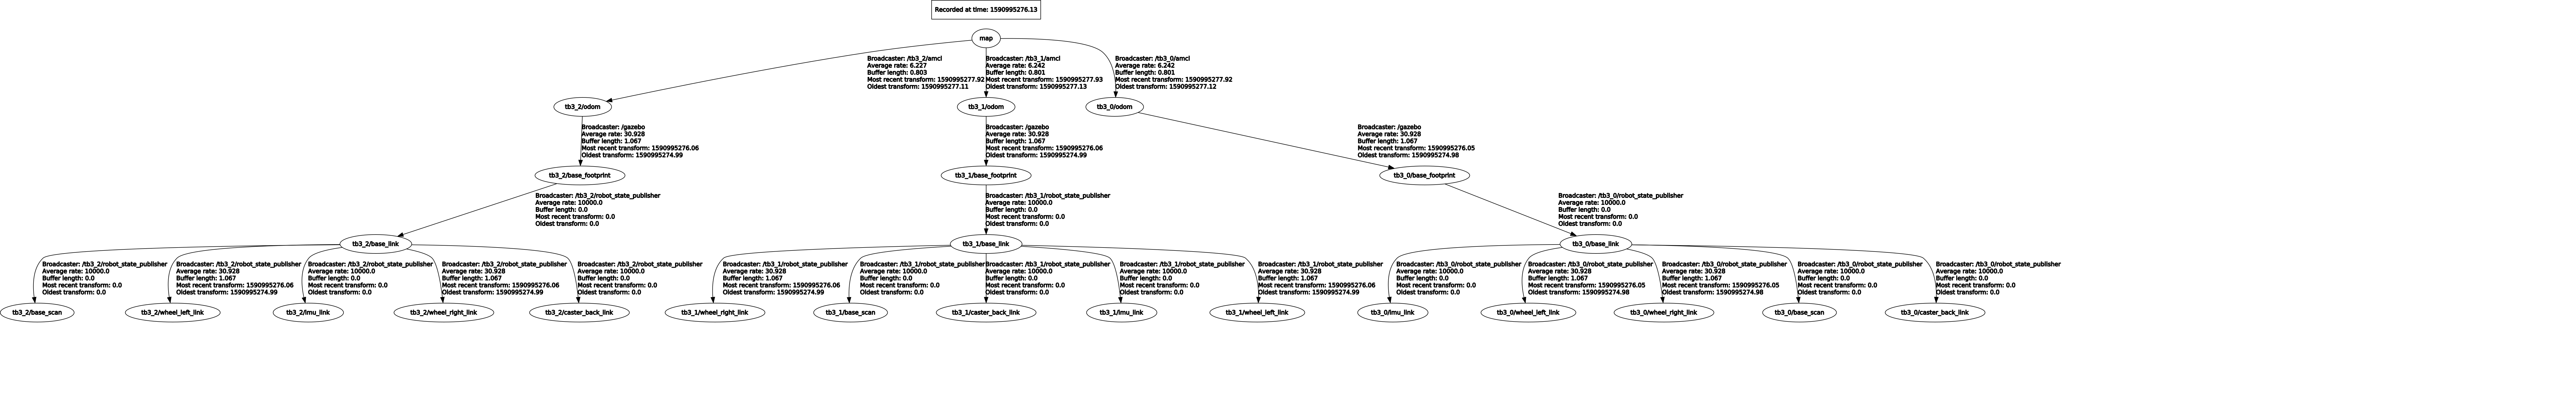
\includegraphics[width = 1.0\textwidth]{content/images/ch2/rqt_tree.png}
        \caption{rqt\_tf\_tree of Multi-robot Scheduling System}
        \label{fig:tf_tree}
        \end{figure}
       
    \item \textbf{rqt\_graph.} rqt\_graph is a type of rqt. It is a graphical tool that presents the status of nodes and topics. Figure \ref{fig:rqt_graph} presents relation of nodes in Multi-robot Scheduling System.
    \begin{figure}[htbp]
        \centering
        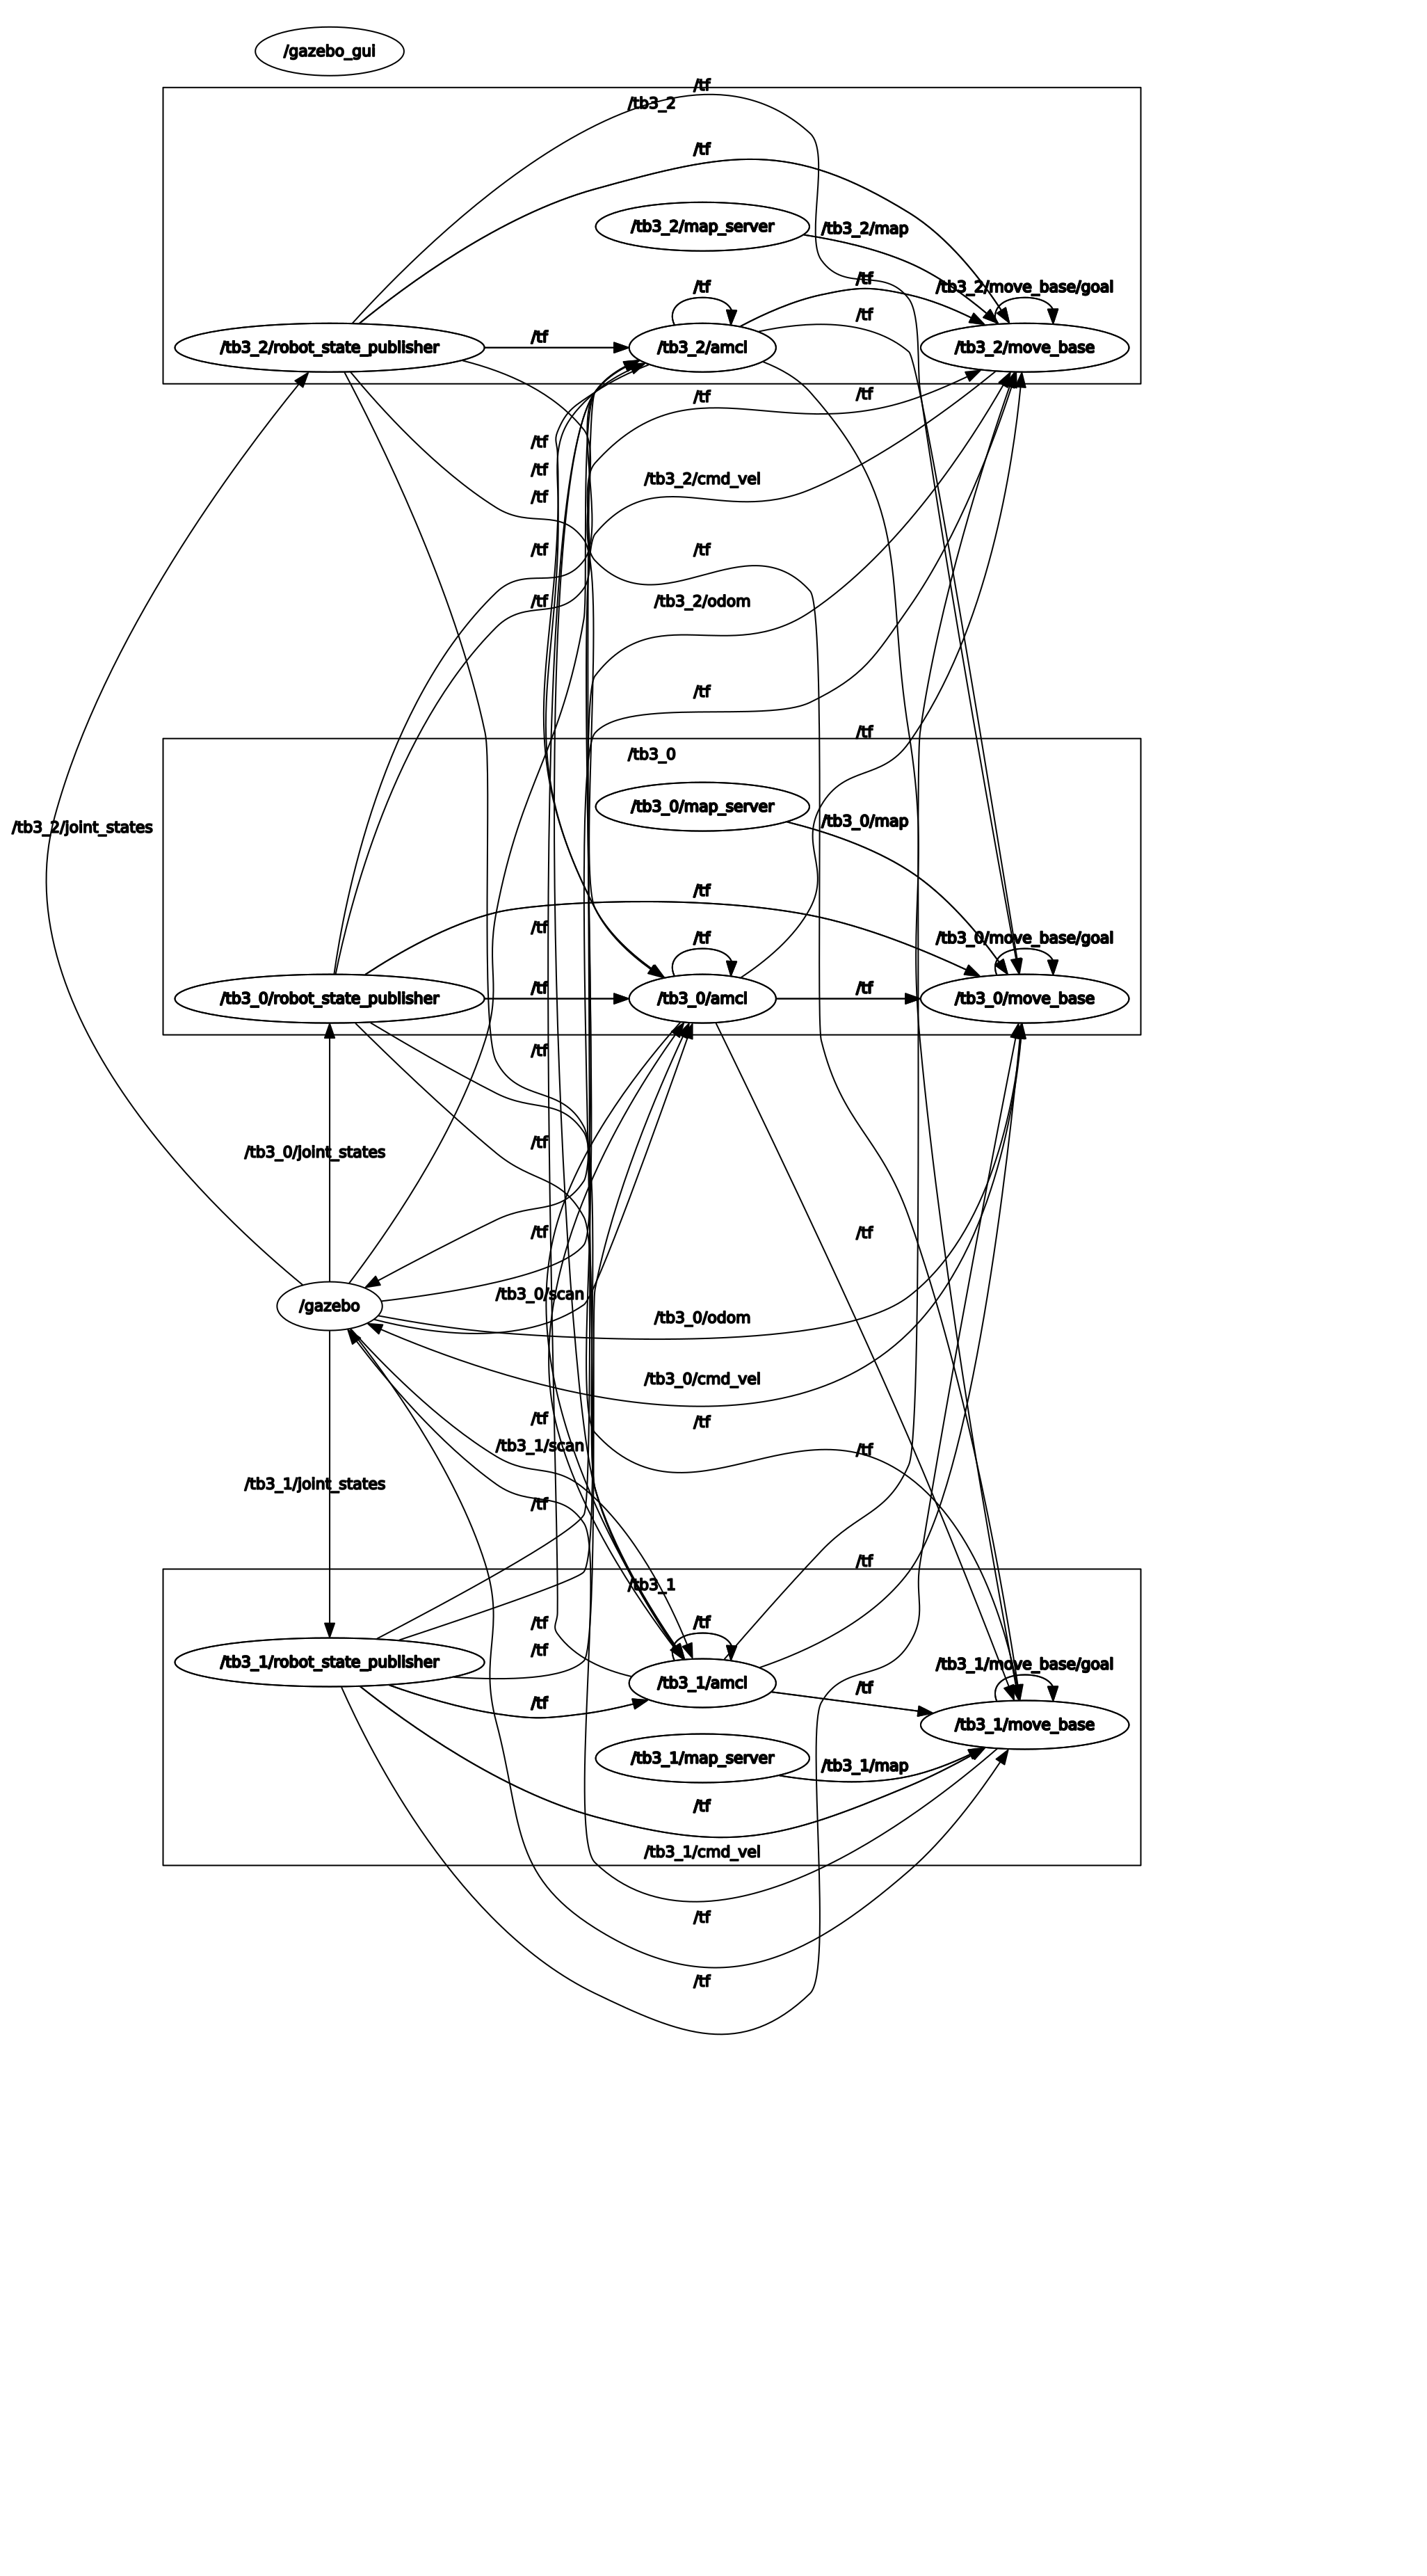
\includegraphics[width = 0.7\textwidth]{content/images/ch2/rosgraph.png}
        \caption{rqt\_graph of Multi-robot Scheduling System}
        \label{fig:rqt_graph}
    \end{figure}

    \item \textbf{Gazebo.} Gazebo \cite{GZ} is the 3D simulation tool intergrated with ROS. The details of gezebo are introduced in Chapter \ref{sec:modeling_gazebo}.
\end{itemize}

\section{TurtleBot3 Simulation Using Gazebo}
\label{sec:modeling_gazebo}

\subsection{Gazebo Simulator}
Robot simulation is essential for robotics research, because it can pre-estimate the performance of robot algorithms before applying it to a real robot \cite{Afanasyev2015}. 
The simulatior used in this project is Gazebo. Gazebo is a 3D dynamic indoor and outdoor multi-robot simulator intergrated with ROS, and it offers physics simulation at a much higher degree of fidelity, a suite of sensors, and interfaces for both users and programs \cite{GZ}. 
Using Gazebo simulatior affords to create new 3D model with geometrical primitive or import existing simulated robots and environments. 

\subsection{TurtleBot3 Robot}
The robot model used in this project is TurtleBot3 Burger. Because it is a small, affordable, programmable ROS-based mobile robot for use in research and prototyping. 
As is shown in Figure \ref{fig:robot_hardware}, the basic components are actuators, an SBC (Single-Board Computer) for operating ROS, a LDS sensor for SLAM (Chapter \ref{sec:navigation}) and navigation, restructurable mechanism, an OpenCR embedded board used as a sub-controller, sprocket wheels that can be used with tire and caterpillar, and a 3 cell lithium-poly battery.
The simulated robot (Figure  \ref{fig:simulated_robot}) has a similar outfit. In addition, Gazebo simulates the robot locomotion and sensor measurements used for localization and navigation, and exports the simulation results to ROS.


\begin{figure}[htbp]
\centering
\begin{minipage}[t]{0.48\textwidth}
\centering
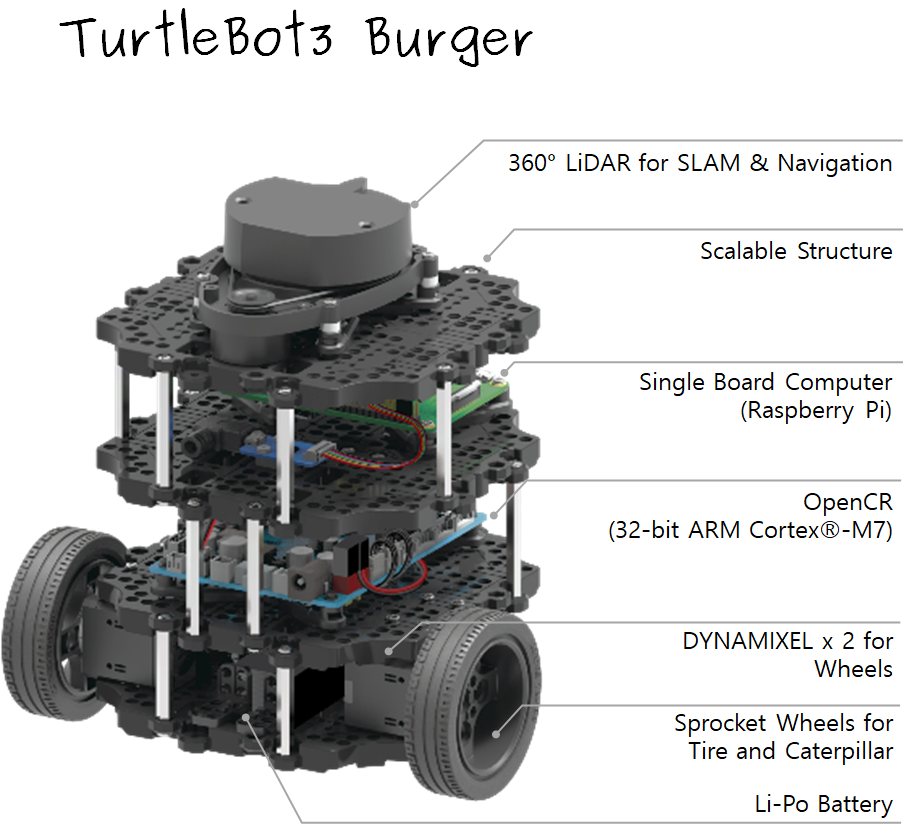
\includegraphics[width=6cm]{content/images/ch2/turtlebot3_burger_components.png}
\caption{Robot Hardware Configuration}
\label{fig:robot_hardware}
\end{minipage}
\begin{minipage}[t]{0.48\textwidth}
\centering
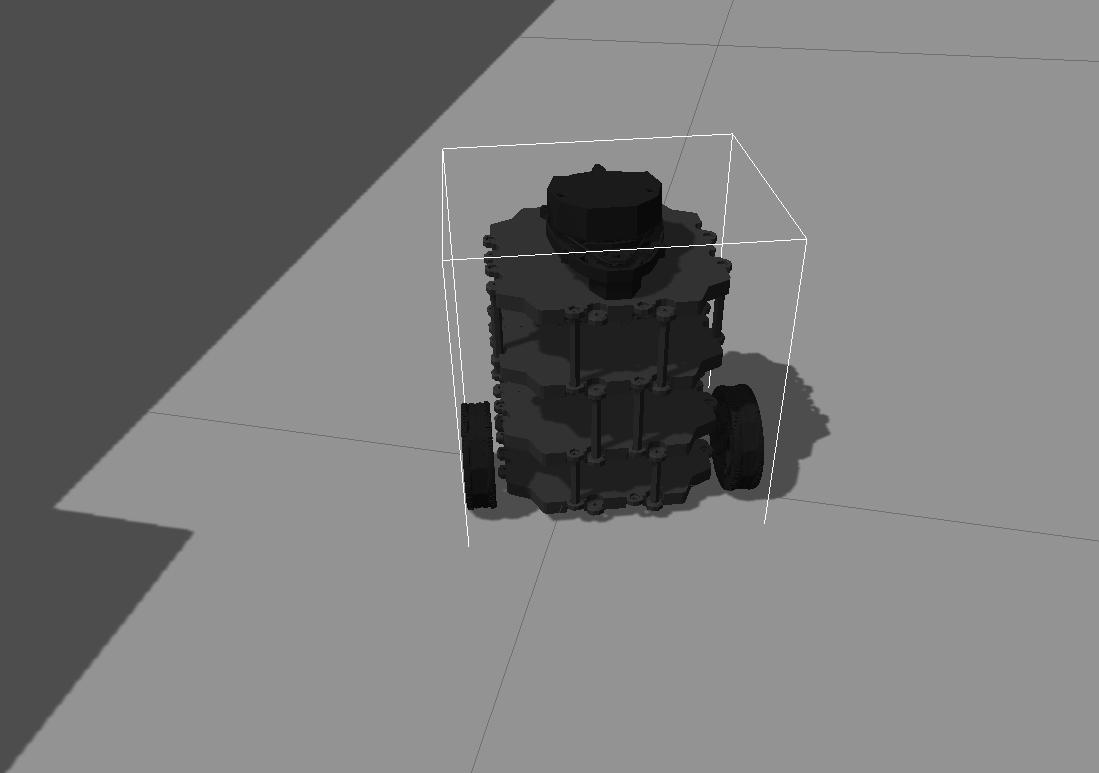
\includegraphics[width=6cm]{content/images/ch2/robot_model.jpg}
\caption{Robot 3D Modeling in Gazebo}
\label{fig:simulated_robot}
\end{minipage}
\end{figure}

\subsection{3D Modeling of Indoor Environment}

In this project we selected a model exactly the same as the floor of the department as a trial 3D model (Figure \ref{fig:modeling_environment_gazebo}).
This model is a typical office enviroment that contains a corridor along the central x-axis and 16 rooms located around the corridor. 

\begin{figure}[htbp]
    \centering
    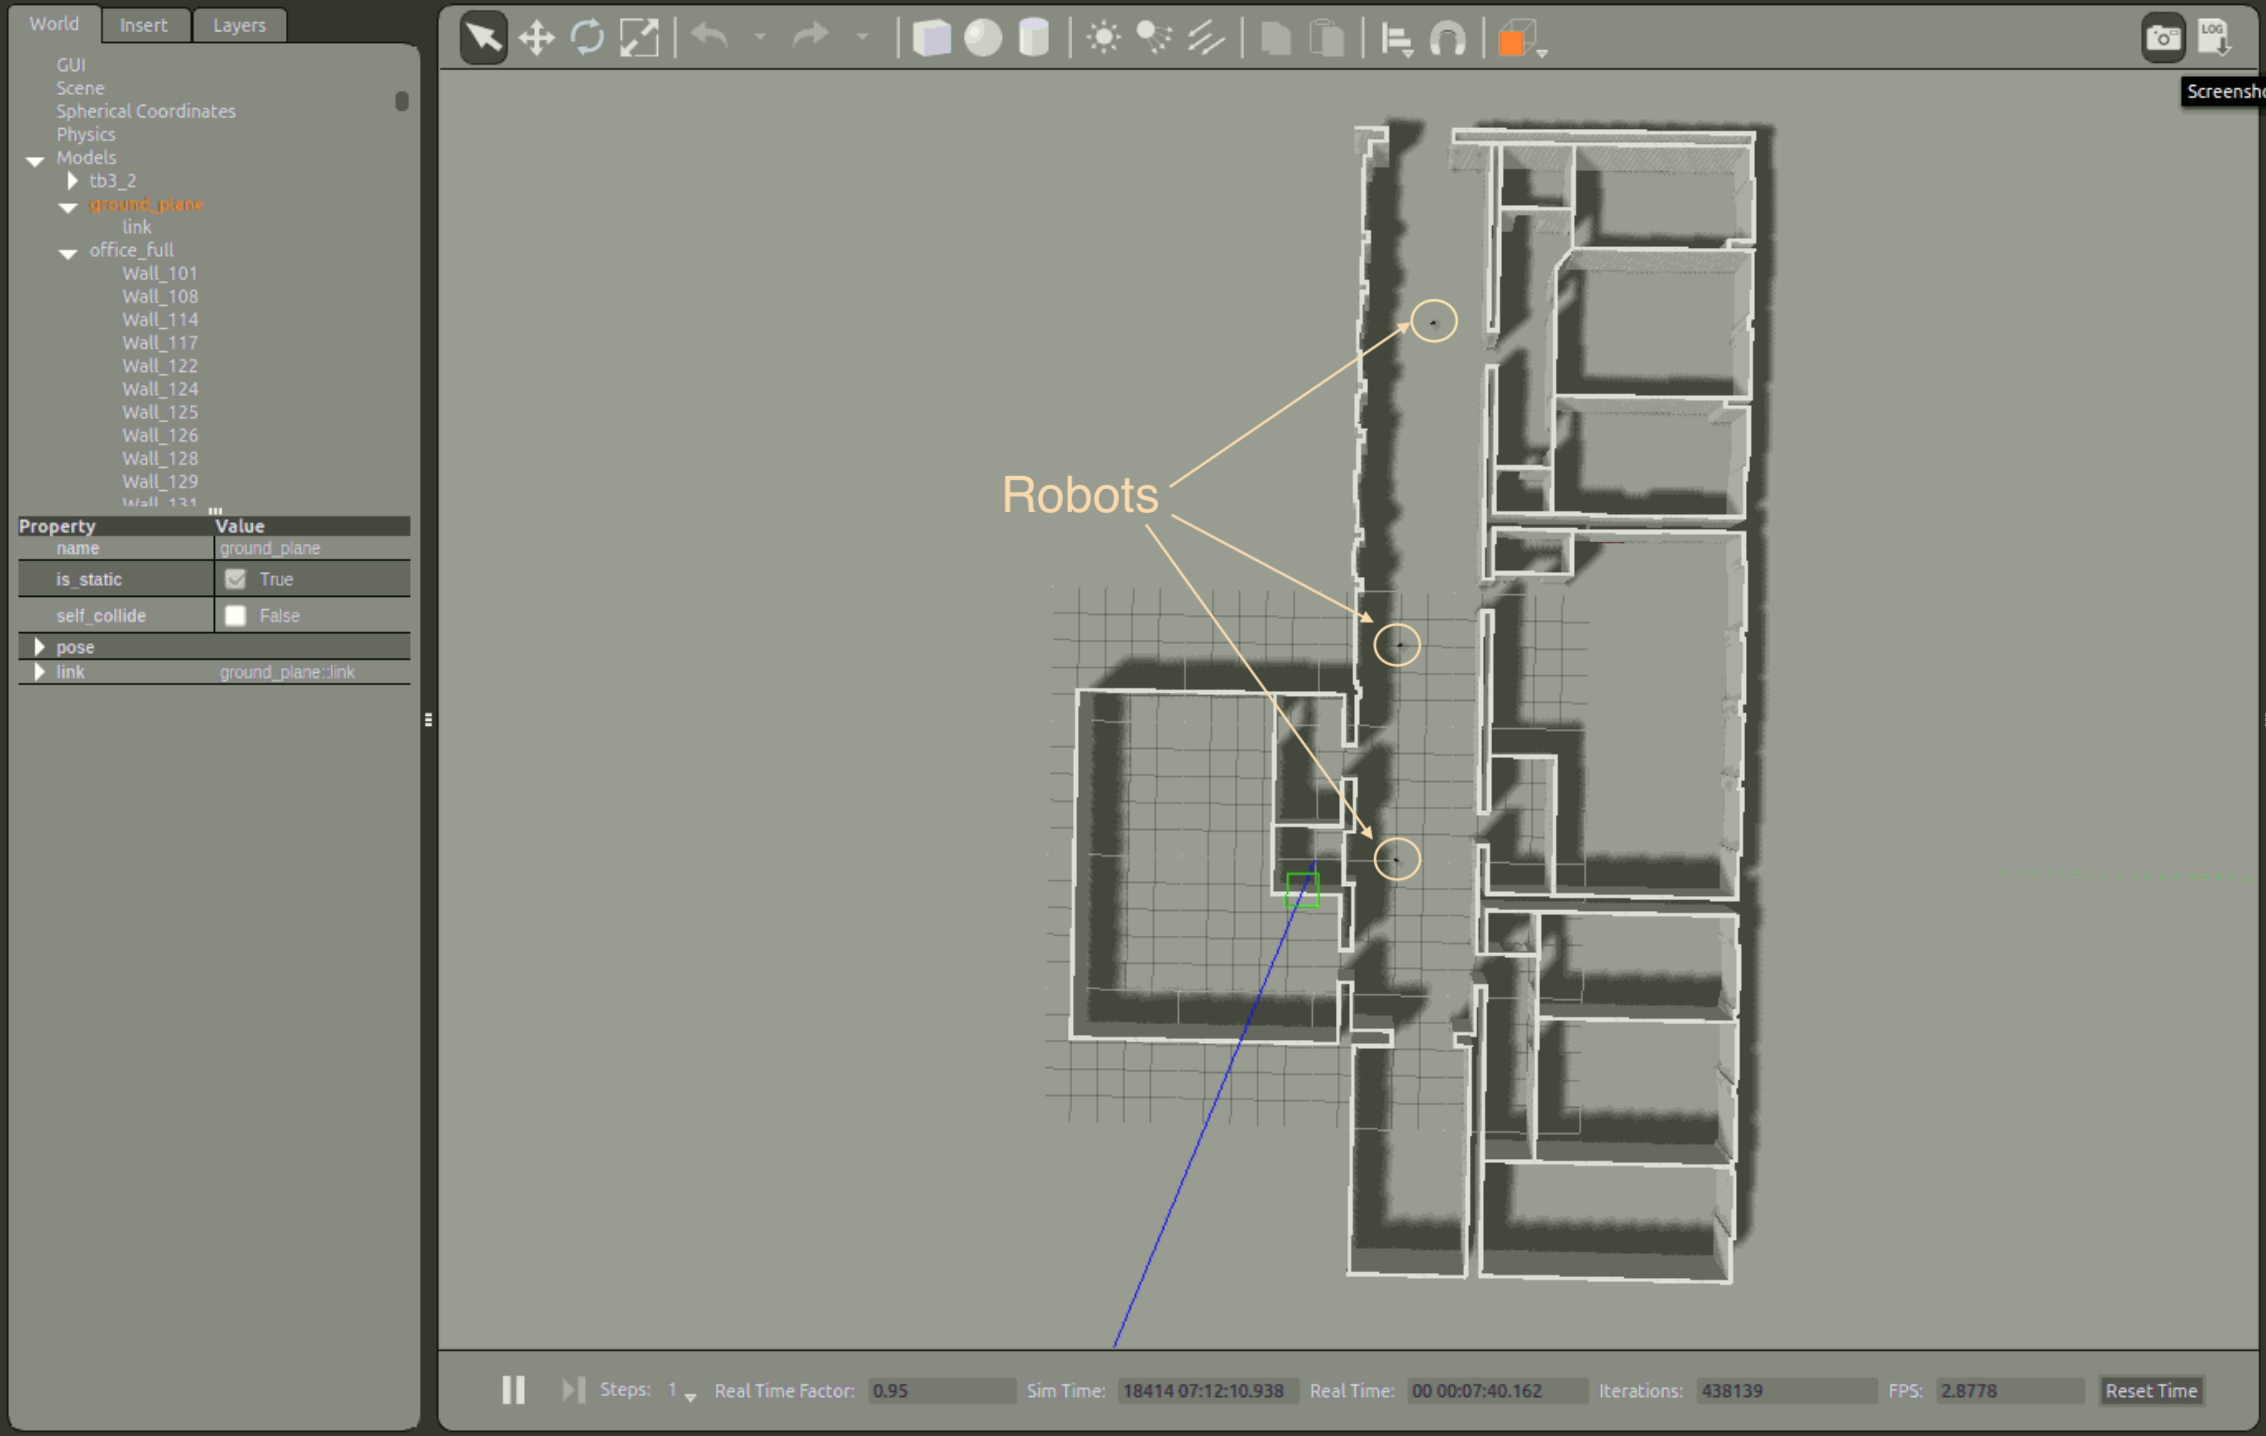
\includegraphics[width = 0.7\textwidth]{content/images/ch2/gazebo_gui_environment.png}
    \caption{3D Modeling of Indoor Environment in Gazebo}
    \label{fig:modeling_environment_gazebo}
\end{figure}

\section{Robot Navigation and Virtual SLAM}
\label{sec:navigation}

There are essential technologies to realize autonomous robot navigation: 
\begin{enumerate}
    \item \textbf{Having map of the given enviroment.} In this project, SLAM(Simultaneous Localization Ana Mapping) is used to create a map of the given enviroment. Using SLAM, the robot explores the unknown spaces and detects its surrounding areas and estimates its current location as well as creating a map. The steps of executing virtual SLAM with TurtleBot3 is shown in Website \cite{T3SLAM}. Once the robot finish exploring the indoor enviroment, an occupancy grid map (OCM) is generated (Figure \ref{fig:occupancy_grid}).
    \item \textbf{Measuring or estimating the pose of robot.} Pose is consists of position and orientation. The dead reckoning \cite{DEADRECKONING} is the most popular indoor pose estimation method for the robot. The amount of movement of robot is measured with the rotation of the wheel. However, the error between th calculated distance with wheel ratation and the actual travel distance increases over time. Therefore, the inertial measurement unit (IMU) sensor\cite{Woojin17} is used to measure triaxis angular velocities and triaxis acceleration to estimate the position of the mobile robot.  This inertial data can be used to compensate the error of position and orientation between calculated value and the actual value.
    \item \textbf{Avoiding obstacles such as walls and furniture.} The laser-based distance sensor on robot are widely used in figuring out whether there are obstables including walls, furniture and other robots. The common laser-based distance sensor inludes LDS (Laser Distance Sensor), LDF (Laser Doppler flowmetry) and LiDAR (Light Detection And Ranging) and ultrasonic sensors and infrared distance sensors. The TurtleBot3 equips 360 Laser Distance Sensor LDS-01. The visualization of Laser data in Rviz is shown in Figure \ref{fig:rviz_gui}.
    \item \textbf{Finding the optimal route calculation and driving.} It is important to find the optimized route to the distination. There are many algorithms that perform path searching and planning such as A* algorithm\cite{ASEARCH}, potential field\cite{POTENTIAL}, particle filte\cite{PARTICLE}, and RRT (Rapidly-exploring Random Tree)\cite{RRT}.
    \begin{figure}[htbp]
        \centering
        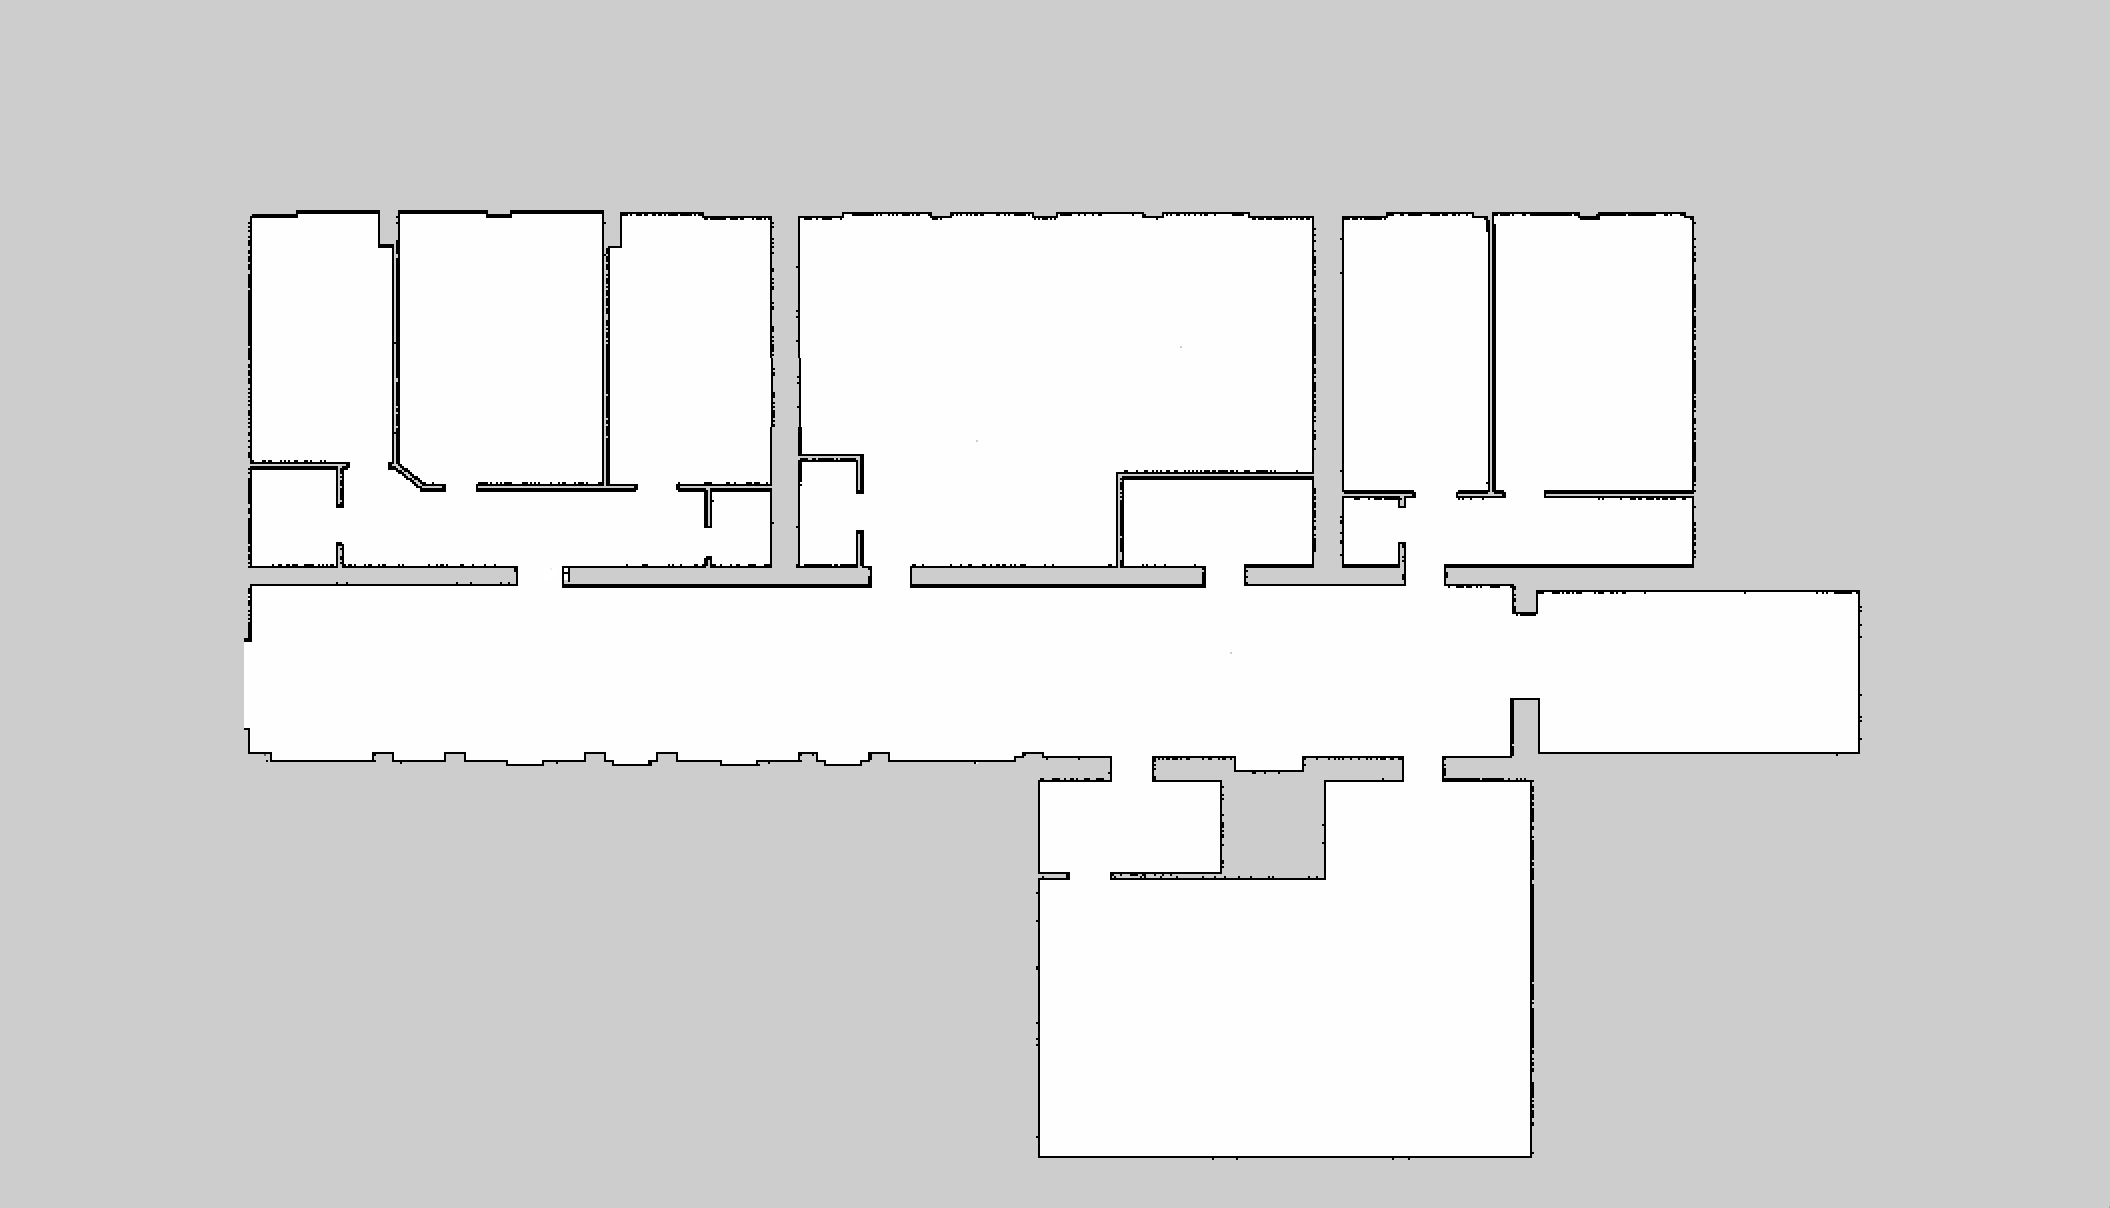
\includegraphics[width = 0.7\textwidth]{content/images/ch2/occupancy_grid.png}
        \caption{Occupancy Grid Map (OGM). White presents the free area in which robots can move, black presents the occupied area in which robots can not move, and gray is the unknown area.}
        \label{fig:occupancy_grid}
    \end{figure}
\end{enumerate}


\section{Exist Task Scheduling Methods}
So far, the background information such as tools and important concepts of ROS are introduced. This Chapter discusses some popular methods of task scheduling. Those task scheduling methods can be divided into centralized methods and distributed methods.

\subsection{Centralized Method vs. Distributed Method}
In the case of centralized method, a centralized schedule collects all task requests and uses resource utilization information to schedule tasks. The centralized method is easy to manager and faster to repair in case of failure. However, the autonomy of the robots in pure centralized method is limited becaued all robots only execute commands from centralized scheduler and not determine what tasks to do \cite{NUNES201755}. In addition, since the centralized scheduler must compute all resources and tasks, it has less scalability which becomes the bottleneck in large-size network \cite{CHRISTODOULOPOULOS20091172}.
Chapter \ref{sec:constraint_programming} introduces a centralized constraint programming method. 

In the case of distributed method, there are multiple distributed schedulers keep tracking the resource availability and use this information to perform task scheduling\cite{CHRISTODOULOPOULOS20091172}. This method distributes the associated computation overhead, as a result it eliminates the bottleneck caused by the centralized scheduler and improves the scalability and realiability and scalability if the network. The challenge in distribute method is the coordination of distribute schedulers as well as the required control plane overhead \cite{CHRISTODOULOPOULOS20091172}.
Chapter \ref{sec:auction_method} introduces a distributed auction method and Chapter \ref{sec:distributed_capability_based_method} introduces a distributed capability-based method.

\subsection{Centralized Constraint Programming Method}
\label{sec:constraint_programming}

Booth proposed a multi-robot system that support elderly residents in a retirement home setting in  \cite{retire2017}. The robots search for elderly residents in the enviroment in the morning, eliciting their availability and preferences for activities. The centralized scheduler then use constraint programming method to allocate these assistive activities over the day. Those problem-specific constrains includes robot energy consumption, activity priority, robot-user activity synchronization, user location, and user availability carlendar that identifies their busy intervals. Once this information is attained, the system allocate and schedule activities to robots for the day before executing the plan.

In addition, there are other centralized methods such as centralized mixed-integer programming \cite{Korsah13}.

\subsection{Distributed Capability-based Method}
\label{sec:distributed_capability_based_method}
Kim proposed a distributed capability-based method \cite{KIM2016386}. This method is designed to allow robots to perform resonable decision-making when they can handle the new task as well as tasks in its queue.
In this method, the scheduler sends a query to all robots to get a list of capability for the tasks. Then it selct one robot with the best capablility to delegate, and then send instruction and deadline to the selected robot. Besides, the robot capability to a task varies from [0,1]. This value determins how well the robot can handle the new task by deadline while taking care of current tasks.


\subsection{Distributed Auction Method}
\label{sec:auction_method}
When system perform a long-term task alloacation process, the communication link between costumer agent and robots may be disconnected. This may couse a conflict or failed assignment. 
Distributed methods are more suitable in this case as distribute the computation to individual agents \cite{NUNES201755}. 
Dong-Hyun Lee proposed a resource-oriented, distributed auction algorithm \cite{Dong2015}. 
The customer agents and robots with limited communication ranges construct an ad-hoc network tree. The customer agent becomes auctioneer and broadcasts an auction call to the task. The robots become bidders and submit their bid values to the customer agent. The bid values consider local information such as the tasks in robot task queue, robot's resource levels and estimated travel distance and time for multiple path. 
Since each path consists of different charging stations, the robot's resource levels after completing a task and estimated travel time depends on the path. 
After receiving all bid values, the agent assigns the task to the robot with the lowest bid value. 
This senario has many advantages. It is more efficient communication overhead and energy efficiency. To be more precise, it not only avoids unexpected battery drain while robot processing task, but also let robots maintain high capacities. In addition, in distributed method, robots don't need to broadcast its information such as current position and battery levels frequently. Therefore, compared to centralized methods, distributed method not only avoids unnecessary communication but also improves robot autonomy \cite{Shah07}.


\section{Exist Quantities of Cost Function}
\label{sec:cost_function}
One of the most important steps when designing a multi-robot task scheduling algorithm is determin the costs of tasks. Jia summaries several physical quantities used in algorithm's cost in \cite{Jia2013ASA}. In their study it can be concluded that the most common used decision variables are estimated travel distance and time, as proposed in \cite{Dong2015}. Other kinds of decision variables involved are the number of traversals and energy consumed. 
In addition, Korsah proposed a comprehensive taxonnomy of multi-robot task scheduling problems that explicitly takes into consideration the issues of interrelated utilities and constraints. In this taxonnomy, tasks are distinguished by decomposability and multi-agent-allocatability \cite{Korsah13}.
